\chapter{Implementación}

\section{Herramientas}

En esta sección se describen las distintas herramientas empleadas durante el desarrollo del proyecto, indicando la función que desempeña cada una de ellas en las distintas fases de creación e implementación de la aplicación.

\begin{itemize}
    \item \textbf{Visual Studio Code:} Entorno de desarrollo integrado \textit{(IDE)} utilizado para la implementación del Frontend de la aplicación.
    \item \textbf{Android Studio:} Herramienta empleada para la ejecución y prueba de la aplicación en emuladores y dispositivos Android, permitiendo visualizar los cambios realizados durante el desarrollo.
    \item \textbf{Supabase:} Plataforma Backend as a Service \textit{(BaaS)} utilizada como backend de la aplicación, proporcionando servicios de base de datos, autenticación y almacenamiento.
    \item \textbf{Jira:} Herramienta de gestión de proyectos utilizada para la planificación y organización de los distintos sprints, facilitando la distribución y seguimiento de las tareas.
    \item \textbf{Github:} Plataforma de control de versiones empleada para alojar el \href{https://github.com/ntsec7/TFG}{código fuente del proyecto} y gestionar su evolución mediante un repositorio.
    \item \textbf{Google Drive:} Servicio de almacenamiento en la nube utilizado en la generación de los distintos diagramas representados en el presente documento.
    \item \textbf{Overleaf:} Plataforma basada en \LaTeX{} utilizada para la redacción y edición de la presente memoria.
    \item \textbf{Figma:} Herramienta de diseño empleada en la elaboración de los diagramas de interfaz de usuario incluidos en el documento.
    \item \textbf{Gmail:} Servicio de correo electrónico utilizado para el envío de mensajes de verificación de las cuentas registradas en la aplicación y para la confirmación de los cambios de contraseña.
\end{itemize}    

\section{Explicación de la implementación}

El proceso más importante e interesante de la aplicación es la toma de decisiones. Para la creación de una decisión se utilizan dos modelos auxiliares, \textit{DecisionDraft} y \textit{OptionDraft}, que contienen los mismos campos que los modelos \textit{Decision} y \textit{Option} respectivamente, pero sin los identificadores asociados. Estos modelos tienen como finalidad almacenar los datos temporalmente entre pantallas. En \textit{DecisionDraft} se almacena además la lista de \textit{OptionDraft} creadas. Una vez finalizado el diseño de la decisión, el usuario puede optar por dos caminos: crear la decisión directamente para ponerla en votación, o iniciar el proceso de sugerencia de opciones. Dependiendo de la elección, tal como se muestra en la Figura~\ref{fig:diugrouphomepage}, la decisión aparecerá en un apartado u otro de la pantalla. \\

Una decisión atraviesa 4 estados a lo largo de su ciclo de vida, tal como podemos observar en la Figura~\ref{fig:ciclodecision}. Durante la creación se encuentra en el estado \textit{Draft}; posteriormente pasa a \textit{Option} (estado que puede omitirse); a continuación, a \textit{Vote}; y finalmente a \textit{Finish}. En las transiciones de \textit{Option} a \textit{Vote} y de \textit{Vote} a \textit{Finish} es posible especificar un tiempo máximo tras el cual el cambio de estado se produce automáticamente. Para ello se ha implementado una \textit{Edge Function} —que permite encapsular operaciones que requieren ejecutarse en el servidor— la cual se ejecuta una vez por minuto y comprueba si la hora de finalización del estado actual es menor o igual que la hora actual, actualizando el estado de la decisión cuando se cumple dicha condición. \\

    \begin{figure}[ht]
        \centering
        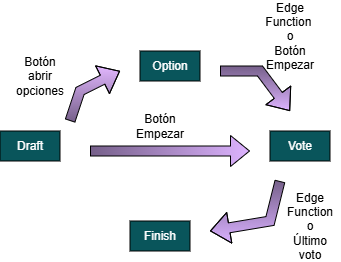
\includegraphics[width=0.7\textwidth]{figuras/EstadosDecision.png}
        \caption{Ciclo de vida de una decisión }
        \label{fig:ciclodecision}
    \end{figure}

Asimismo, cuando una decisión se encuentra en el estado \textit{Vote}, se muestra una pantalla de votación distinta en función de su tipo: \textit{simple}, \textit{ranking} o \textit{roulette}. Una vez que todos los miembros participantes han registrado su voto, la decisión pasa automáticamente al estado \textit{Finish}, aunque no haya expirado el tiempo destinado a la votación. Esto es posible gracias a un \texttt{trigger} que se dispara al registrarse cada nueva votación. Las decisiones de tipo \textit{roulette} no tienen un tiempo máximo entre los estados \textit{Vote} y \textit{Finish}, ya que únicamente requieren que el creador de la decisión acceda a la pantalla de votación. \\

Para que todo lo anterior funcione de forma ordenada y coherente, es necesario que los cambios se reflejen en tiempo real para todos los usuarios. Con este fin, se activa la opción \texttt{Realtime} en las tablas correspondientes de \textit{Supabase} y se obtiene el flujo de datos mediante \texttt{Riverpod} y \texttt{Stream}. \texttt{Riverpod} es una librería que desacopla la lógica de negocio de la interfaz, facilitando una arquitectura reactiva en la que los cambios de estado se propagen automáticamente a los componentes de la UI. Por su parte, \texttt{Stream} abre un canal de datos continuo y sincronizado con la base de datos.